\documentclass[12pt]{article}

\usepackage{amsmath}
\usepackage{multirow}
\usepackage{microtype}
\usepackage{subcaption}
\usepackage{booktabs}
\usepackage{siunitx}
\sisetup{output-decimal-marker = {,}}

\usepackage{graphicx}
\renewcommand{\figurename}{Slika}
\renewcommand{\tablename}{Tabela}

\newcommand{\Ai}{\mathrm{Ai}}
\newcommand{\Bi}{\mathrm{Bi}}
\newcommand{\dd}{\,\mathrm{d}}

\DeclareSIUnit{\mumps}{\micro\meter\per\second}

\setlength\parindent{0pt}

\pagenumbering{arabic}
\setcounter{page}{1}

\begin{document}

\newcommand{\institutionname}{Univerza v Ljubljani}
\newcommand{\projecttitle}{2. Naključni Sprehodi}
\newcommand{\authorname}{Tilen Šket, 28221057}
\newcommand{\instructions}{\textit{
        Napravi računalniško simulacijo dvorazsežne naključne hoje za polete in sprehode. Začni vedno v izhodišču $(x = y = 0)$, nato pa določi naslednjo lego tako, da naključno
        izbereš smer koraka in statistično neodvisno od te izbire še njegovo dolžino, torej
        $p(l) \propto l^{-\mu}$.
        V vsakem primeru nariši nekaj značilnih slik sprehodov za 10, 100, 1000
        in 10 000 korakov. Iz velikega števila sprehodov z velikim številom korakov nato poskusi določiti eksponent $\gamma$ za nekaj izbranih parametrov $\mu$ oziroma funkcij $f(x)$ v posameznih primerih ter presodi, za kakšno vrsto difuzije gre.
    }}
\newcommand{\subjectname}{Matematično-fizikalni praktikum}
\newcommand{\institutionlogo}{UlFmf_logo.pdf}

\begin{titlepage}
    \centering

    \includegraphics[width=0.7\textwidth]{\institutionlogo}

    \vspace{1.0cm}

    \Large
    \textbf{\subjectname}

    \vspace{1.0cm}

    \LARGE
    \textbf{\projecttitle}

    \vspace{1.0cm}

    \Large
    \textbf{\authorname}

    % \vspace{1.0cm}
    \vfill

    \large
    \textbf{Navodila:}

    \vspace{0.5cm}

    \large
    \instructions%

    \vspace{0.5cm}
    \vfill

    \large
    \textbf{\today}

\end{titlepage}

\addtocounter{page}{1}

\newpage
Airyjevi funkciji $\Ai$ in $\Bi$
se v fiziki pojavljata predvsem v optiki in kvantni mehaniki.  Definirani sta kot neodvisni rešitvi enačbe
%
\begin{equation*}
    y''(x) -xy(x) = 0
\end{equation*}
%
in sta predstavljivi v integralski obliki
%
\begin{equation*}
    \Ai(x) = \frac{1}{\pi} \int_0^\infty \cos (t^3/3 + x t) \dd t \>,\quad
    \Bi(x) = \frac{1}{\pi} \int_0^\infty \left[ \mathrm{e}^{-t^3/3 + x t}
        + \sin (t^3/3 + x t) \right] \dd t \>.
\end{equation*}
%

\section{Postopek}
\subsection{Taylorjev razvoj}

Za majhne $x$ lahko funkciji $\Ai$ in $\Bi$ izrazimo
z Maclaurinovima vrstama
%
\begin{equation*}
    \Ai(x) = \alpha f(x) - \beta g(x)\>,\qquad
    \Bi(x) = \sqrt{3}\, \Bigl[\alpha f (x) + \beta g(x) \Bigr]\>,
\end{equation*}
kjer v $x=0$ veljata zvezi
%
$\alpha = \Ai(0) = \Bi(0)/\sqrt{3}\approx 0.355028053887817239$ in
$\beta = -\Ai'(0) = \Bi'(0)/\sqrt{3}\approx 0.258819403792806798$.
Vrsti za $f$ in $g$ sta
\begin{equation*}
    f(x) = \sum_{k=0}^\infty
    \left(\frac{1}{3}\right)_k \frac{3^k x^{3k}}{(3k)!} \>, \qquad
    g(x) = \sum_{k=0}^\infty
    \left(\frac{2}{3}\right)_k \frac{3^k x^{3k+1}}{(3k+1)!} \>,
\end{equation*}
kjer je
\begin{equation*}
    (z)_n = \Gamma(z+n)/\Gamma(z) \>, \qquad (z)_0 = 1 \>.
\end{equation*}
Zapišimo Maclaurinovi seriji za naši funkciji rekurzivno. Za $f(x) = \sum_{\rm k=0}^{\inf} a_{\rm k}$ $g(x) = \sum_{\rm k=0}^{\inf} b_{\rm k}$. Velja
\begin{align}
    a_{\rm k} & = a_{\rm k-1} \frac{(k-2) x^3}{3k};   & a_0   = 1, \\
    b_{\rm k} & = b_{\rm k-1} \frac{(k-1) x^3}{3k+1}; & b_0 = x.
\end{align}

Z izraženima rekurzivnima enačbama lahko funkcijo dobro aproksimiramo v okolici izhodišča. To sem naredil in prikazal na sliki (\ref{fig:NapakeTaylor}). Iz tega grafa vidimo približno območje, kjer lahko za naša željeno natančnost še vedno uporabljamo Taylorjev razvoj, jaz sem si za to območje izbral med $\num{-28}$ in $\num{10}$ za $\Ai$ in med $\num{-28}$ in $\num{26}$ za $\Bi$.

\begin{figure}
    \centering
    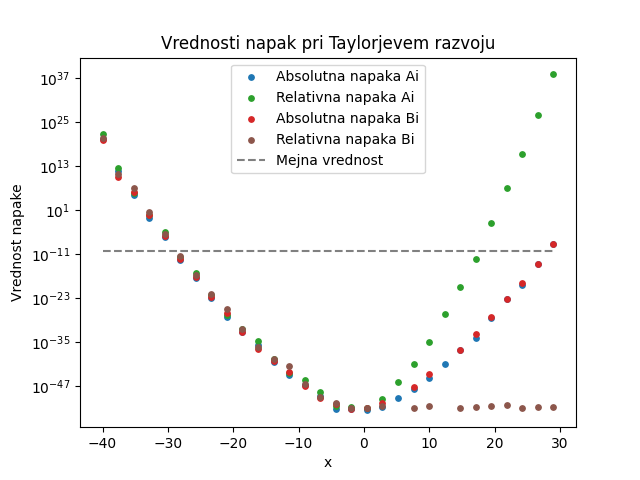
\includegraphics[width=0.7\textwidth]{NapakeTaylor.png}
    \caption{\label{fig:NapakeTaylor} Vrednosti absolutne in relativne napake nekaterih točk med -40 in 40. Opazimo, da aproksimacija res dobro deluje le v okolici izhodišča, kot pričakovano. Le relativna napaka funkcije $\Bi$ ostane majhna, kar je posledica tega, da funkcija raste preko vseh meja v pozitivni neskončnosti.}
\end{figure}

\newpage
\subsection{Asimptotski razvoj}
Za velike vrednosti $|x|$ Airyjevi funkciji aproksimiramo
z njunima asimp\-tot\-ski\-ma razvojema.  Z novo spremenljivko
$\xi=\frac{2}{3} |x|^{3/2}$ in asimptotskimi vrstami
%
\begin{equation*}
    L(z) \sim \sum_{s=0}^\infty \frac{u_s}{z^s}\>,\qquad
    P(z) \sim \sum_{s=0}^\infty (-1)^s \frac{u_{2s}}{z^{2 s}}\>,\qquad
    Q(z) \sim \sum_{s=0}^\infty (-1)^s \frac{u_{2s+1}}{z^{2 s+1}}\>,
\end{equation*}
s koeficienti
\begin{equation*}
    u_s = \frac{ \Gamma(3s + \frac{1}{2})}
    {54^s s!\, \Gamma(s + \frac{1}{2}) }
\end{equation*}
za velike pozitivne $x$ izrazimo
%
\begin{equation*}
    \Ai(x)\sim  \frac{\mathrm{e}^{-\xi}}{2\sqrt{\pi} x^{1/4}} \, L(-\xi) \>, \qquad
    \Bi(x)\sim  \frac{\mathrm{e}^{\xi}} { \sqrt{\pi} x^{1/4}} \, L(\xi)\>,
\end{equation*}
%
za po absolutni vrednosti velike negativne $x$ pa
%
%
\begin{align*}
    \Ai(x) & \sim  \frac{1}{\sqrt{\pi} (-x)^{1/4}}
    \Bigl[ \phantom{-}\sin(\xi-\pi/4) \, Q(\xi)
    + \cos(\xi-\pi/4) \, P(\xi)\Bigr] \>,          \\
    \Bi(x) & \sim  \frac{1}{\sqrt{\pi} (-x)^{1/4}}
    \Bigl[ - \sin(\xi-\pi/4) \, P(\xi)
        + \cos(\xi-\pi/4) \, Q(\xi)\Bigr]\>.
\end{align*}
Ponovno zapišemo člene naših vrst rekurzivno in dobimo:
\begin{align*}
     & L: a_{\rm k}     = a_{\rm k-1} \frac{(3k-0.5) (3k-2.5)}{18k x}                                                                \\
     & P: b_{\rm 2k}    = - b_{\rm 2k-2} \frac{(6k-0.5)(6k-1.5)(6k-2.5)(6k-3.5)(6k-4.5)(6k-5.5)}{54^2 2k (2k-1)(2k-0.5)(2k-1.5) x^2} \\
     & Q: c_{\rm 2k+1}  = - c_{\rm 2k -1} \frac{(6k+2.5)(6k+1.5)(6k+0.5)(6k-0.5)(6k-1.5)(6k-2.5)}{54^2 (2k+1)2k(2k+0.5)(2k-0.5) x^2} \\
     & a_0 = 1, b_0 = 1, c_0 = \frac{5}{72x}
\end{align*}

Te enačbe lahko uporabimo pri implementaciji aproksimacije naših funkcij daleč od izhodišča. Za negativne in pozitivne vrednosti se razlikujejo, zato sem napake izrisal na vsak graf za svoj predznak na slikah (\ref{fig:NapakeNeg}) in (\ref{fig:NapakePoz}). Rezultati tukaj zgledajo dobri, posebej bi povdaril le prelom pri modeliranju funkcije $\Bi$ pri visokih vrednostih $x$, saj tam absolutna napaka ponovno narašča, za kar menim, da je krivo dejstvo, da sama funkcija močno narašča in zato tudi napaka, saj ni dovolj mest za natančno računanje. Več o tem v delu z zlepki.

\begin{figure}
    \centering
    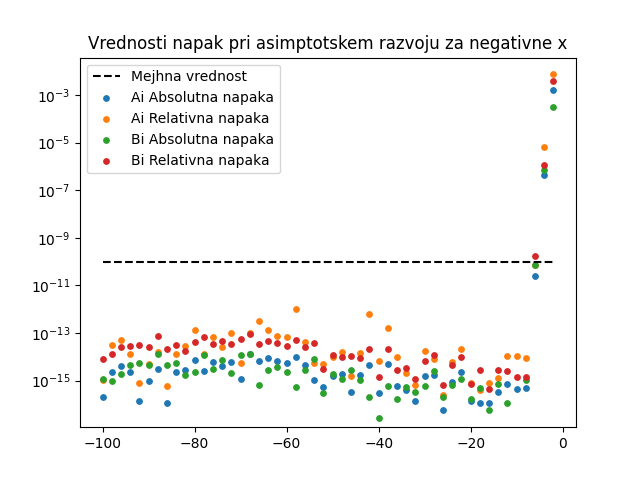
\includegraphics[width=0.7\textwidth]{NapakeAsimptotskoNeg.png}
    \caption{\label{fig:NapakeNeg} Vrednosti absolutne in relativne napake nekaterih točk med -100 in 5. Opazimo, da aproksimacija deluje dobro, dokler je x dovolj negativen, v okolici izhodišča pa napake močno narastejo.}
\end{figure}
\begin{figure}
    \centering
    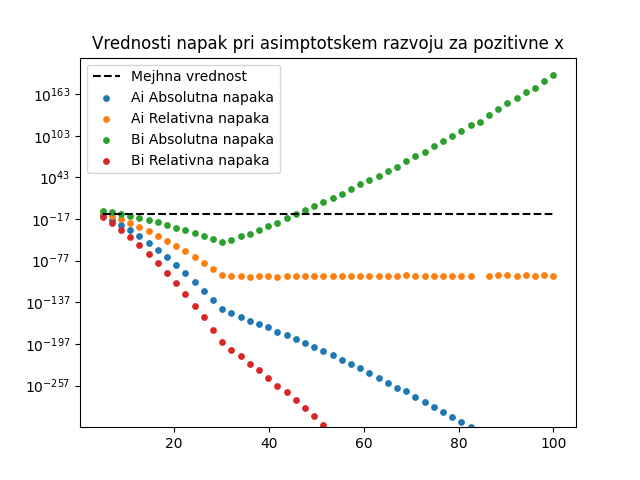
\includegraphics[width=0.7\textwidth]{NapakeAsimptotskoPoz.png}
    \caption{\label{fig:NapakePoz} Vrednosti absolutne in relativne napake nekaterih točk med 5 in 100. Aproksimacija izgleda, da deluje dobro na dovoljšnji oddaljenosti od 0, dokler ne pridemo do preloma pri absolutni napaki $\Bi$, za kar je kriva narava funkcije, ki raste preko vseh meja in pri izračunu numam dovolj mest, da bi absolutna napaka ostala majhna. Več o tem v delu o zlepkih.}
\end{figure}

\subsection{Zlepek}
Tri dele aproksimacije nato zlepimo skupaj, tako da napako na celotnem (oz.\ vsaj čim večjem) območju omejimo pod 10 decimalno mesto. Za točke zlepka sem se sam odločil pri $\num{-28}$ za obe funkciji in $\num{10}$ za $\Ai$ ter $\num{26}$ za $\Bi$. Dobljenima funkcijama sem nato izračunal napaki pri treh različnih decimalne natančnosti, in sicer pri 100, 200 in 500 mestih natančnosti pri računanju. To vidimo na sliki (\ref{fig:Zlepki}). Opazimo, da se koleno premika proti višjim vrednostim x pri višji uporabljeni natančnosti.

\begin{figure}
    \centering
    \begin{subfigure}{0.45\textwidth}
        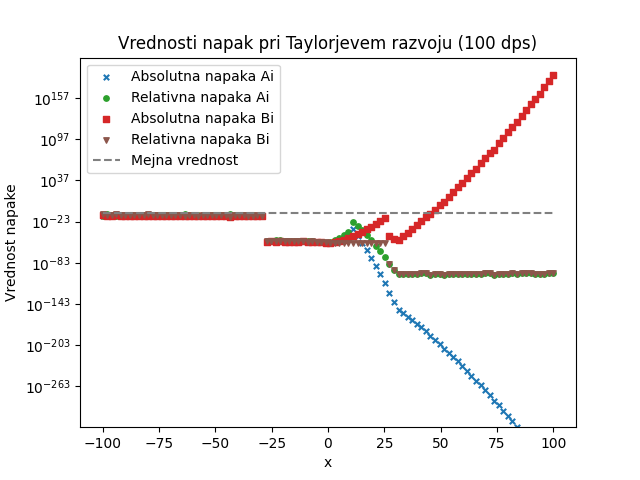
\includegraphics[width=\textwidth]{NapakeZlepek100.png}
    \end{subfigure}
    \begin{subfigure}{0.45\textwidth}
        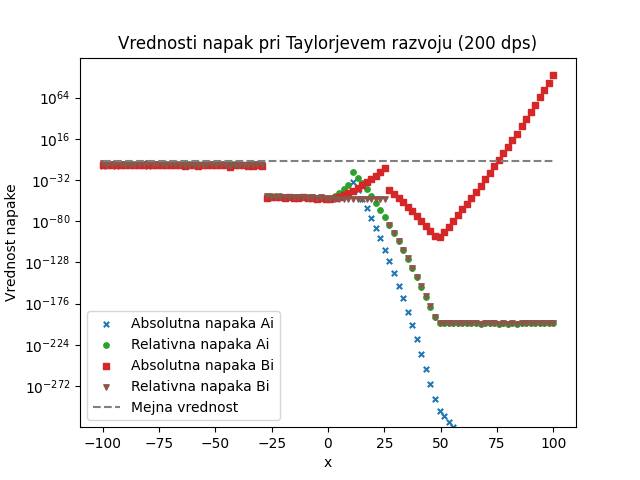
\includegraphics[width=\textwidth]{NapakeZlepek200.png}
    \end{subfigure}
    \begin{subfigure}{0.45\textwidth}
        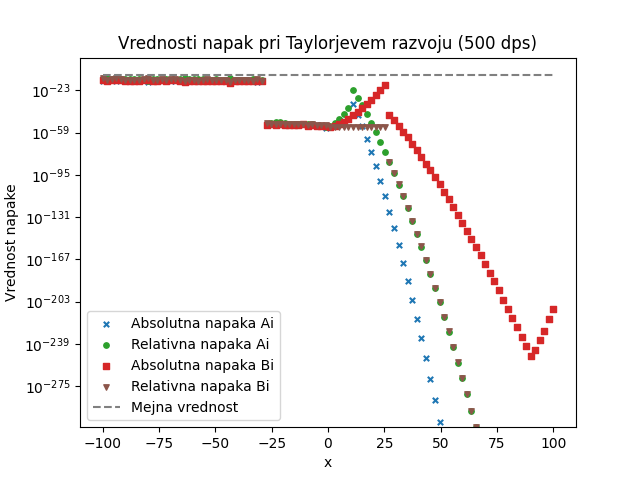
\includegraphics[width=\textwidth]{NapakeZlepek500.png}
    \end{subfigure}
    \caption{\label{fig:Zlepki} Napake modeliranih funkcij in značilno koleno pri visokih vrednostih x za funkcijo $\Bi$. Uporabljena natančnost pri računanju je bila 100, 200 in 500 decimalnih mest. Opazimo premikanje kolena pri različnih natančnostih.}
\end{figure}

\par
Dodajam še graf modeliranih Airyevih funkcij na območju med -30 in 3 na sliki (\ref{fig:graf}). Dodal bi tudi še nekaj optimizacijskih podatkov. Za optimizacijo mislim, da bi se lahko še precej bolj potrudil, vendar je bilo za namene izračuna potrebovane natančnosti kar sem dosegel dovolj. In sicer traja izračun 200 točk med -100 in 100 posamezne funkcije nekaj stotink pod $\SI{3}{\second}$.

\begin{figure}
    \centering
    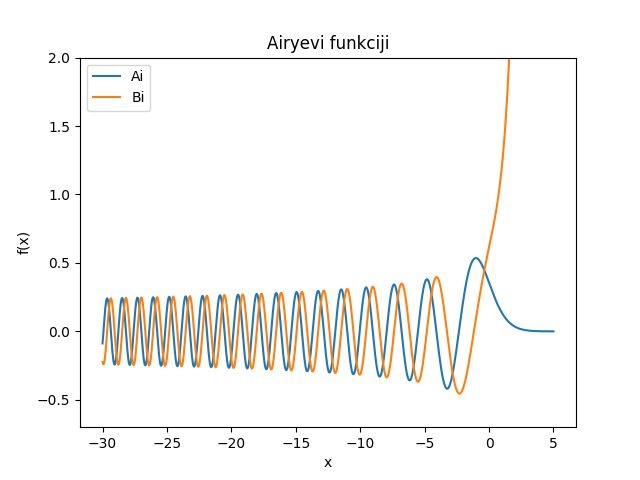
\includegraphics[width=0.7\textwidth]{Graf.png}
    \caption{\label{fig:graf} Graf modeliranih Airyevih funkcij.}
\end{figure}

\newpage
\section{Zaključek}
Najtežji del te naloge bi rekel, da se je bilo znova in znova izmakniti napakam pri relativno enostavnih korakih. Gledano celotno mislim, da sem uspel nalogo rešiti s precej malo teh napak, najbolj očitni pa sta bili večkratne napačne izpeljave rekurzivnih zvez in zgrešena absolutna vrednost pri primerjavi velikosti členov asimptotske vrste.

\par
Še nekaj časovnih statistik. Nalogo sem pričel reševati v petek in ob uspehu, da sem imel, vsaj iz moje takratne perspektive, po 4 urah dela že polovico naloge narejene, kasneje sem ugotovil, da uspešen Taylorjev razvoj ni polovica naloge, sem optimistično in podzavestno zmanjšal nivo nujnosti dela in zato pišem tale zaključek v sredo popoldne v naglici pred odhodom na rojstnodnevno zabavo. Drugi del naloge, vsaj po moji naivni predpostavki, mi je vzel 6 ur intenzivnega dela, kar ne zveni hudo, vendar je bil poleg tega še čas razglabljanja o mojem in postopku drugih. Nadaljno uro sem porabil še za zapis tega poročila, tako da bi ocenil moj skupen čas porabljen za prvo nalogo na dobrih 12 ur dela.
\end{document}
